\section{乘积的性质}\label{sec:geometric-properties-of-products}

先用下面这个关于不可约性的核心结论, 开始研究乘积的几何性质. 它对于研究乘积的维数和光滑性都有用.

\begin{Proposition}{不可约簇的乘积不可约}\leavevmode\label{prop:product-of-irreducible-varieties-is-irreducible}
若 $X$ 和 $Y$ 为不可约仿射簇, 则 $X\times Y$ 不可约.
\end{Proposition}

着手证明之前, 先看几个具体例子, 了解不可约性与乘积之间的关系.

\begin{Example}{不可约的乘积}\leavevmode\label{ex:irreducible-parabola-product}
若 $X=\mathcal{V}(y-x^{2})\subseteq\mathbb{A}^{2}$ 且 $Y=\mathcal{V}(z-1)\subseteq\mathbb{A}^{1}$, 则 $X$ 和 $Y$ 都不可约, 而乘积
\[
  X\times Y=\mathcal{V}(y-x^{2},z-1)\subseteq\mathbb{A}^{3}
\]
是 $\mathbb{A}^{3}$ 中的一条抛物线. $X\times Y$ 的不可约性可以由同构 $X\times Y\cong X$ 看出, 这个同构就是垂直投影 $\mathbb{A}^{3}\to\mathbb{A}^{2}$ 的限制.
\end{Example}

\begin{Example}{可约的乘积}\leavevmode\label{ex:reducible-cross-times-line}
令 $X=\mathcal{V}(xy)\subseteq\mathbb{A}^{2}$ 且 $Y=\mathbb{A}^{1}$. 那么 $X=\mathcal{V}(x)\cup\mathcal{V}(y)$ 是可约的, 乘积也可约:
\[
  X\times Y=\mathcal{V}(x)\cup\mathcal{V}(y)\subseteq\mathbb{A}^{3},
\]
如\hyperref[fig:axes-times-line-intersecting-planes]{下图}所示.
\par\smallskip
{\centering\phantomsection\label{fig:axes-times-line-intersecting-planes}%
  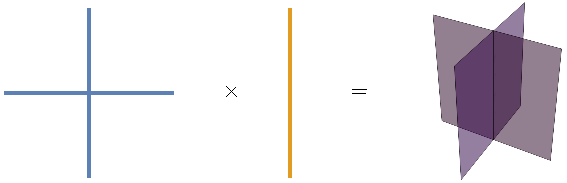
\includegraphics[width=.85\linewidth]{figures/axes-times-line-intersecting-planes.pdf}\par}

尽管 $Y$ 是整个仿射空间, 因而这个例子大为简化, 它仍体现了 Proposition~\ref{prop:product-of-irreducible-varieties-is-irreducible} 的证明要点: 若 $Y$ 不可约, 则把 $X\times Y$ 分解成两个仿射簇的并, 只能来自把 $X$ 作类似的分解.
\end{Example}

\begin{Proof}\textbf{of Proposition~\ref{prop:product-of-irreducible-varieties-is-irreducible}.}\quad
设 $X\subseteq\mathbb{A}^{m}$ 和 $Y\subseteq\mathbb{A}^{n}$ 为不可约仿射簇. 为证明 $X\times Y$ 不可约, 要说明对仿射簇 $Z_{1},Z_{2}\subseteq X\times Y\subseteq\mathbb{A}^{m+n}$, 只有当 $Z_{1}=X\times Y$ 或 $Z_{2}=X\times Y$ 时, 才能有
\begin{equation}\label{eq:product-as-union-of-two-varieties}
  X\times Y=Z_{1}\cup Z_{2}.
\end{equation}

设 \eqref{eq:product-as-union-of-two-varieties} 成立. 对每一点 $a\in X$, 考虑集合
\[
  \{a\}\times Y\subseteq X\times Y.
\]
例如, 若 $X\times Y$ 是 Example~\ref{ex:product-circle-line-cylinder} 的圆柱面或 Example~\ref{ex:reducible-cross-times-line} 的相交平面, 那么集合 $\{a\}\times Y$ 就是乘积中的那些垂直直线. 每个集合 $\{a\}\times Y$ 都是仿射簇 (因为 $\{a\}$ 和 $Y$ 都是仿射簇), 且它们都同构于 $Y$. 因此 $Y$ 不可约意味着对所有 $a\in X$, $\{a\}\times Y$ 不可约. 将 \eqref{eq:product-as-union-of-two-varieties} 两边与 $\{a\}\times Y$ 相交, 得
\[
  \{a\}\times Y
    =\bigl((\{a\}\times Y)\cap Z_{1}\bigr)\cup
     \bigl((\{a\}\times Y)\cup Z_{2}\bigr).
\]
由于 $\{a\}\times Y$ 不可约, 必有
\[
  (\{a\}\times Y)\cap Z_{1}=\{a\}\times Y
  \quad\text{或}\quad
  (\{a\}\times Y)\cap Z_{2}=\{a\}\times Y.
\]
换句话说, 对任意 $a\in X$, 或者 $\{a\}\times Y\subseteq Z_{1}$, 或者 $\{a\}\times Y\subseteq Z_{2}$. 因此, 定义两个集合
\[
  X_{1}=\{a\in X\mid\{a\}\times Y\subseteq Z_{1}\}
  \quad\text{且}\quad
  X_{2}=\{a\in X\mid\{a\}\times Y\subseteq Z_{2}\},
\]
就有
\begin{equation}\label{eq:base-as-union-of-full-fiber-loci}
  X_{1}\cup X_{2}=X.
\end{equation}
到此只知道 $X_{1}$ 和 $X_{2}$ 是 $X$ 的子集, 但它们本身实际上也是仿射簇. 为看出这一点, 回忆 $Z_{1}$ 是仿射簇, 因此
\[
  Z_{1}=\mathcal{V}(f_{1},\ldots,f_{r})
\]
其中 $f_{1},\ldots,f_{r}\in K[x_{1},\ldots,x_{m},y_{1},\ldots,y_{n}]$ 为某些多项式. 对任意 $b\in Y$, 考虑仿射簇
\[
  (X_{1})_{b}=\mathcal{V}\bigl(f_{1}(x,b),\ldots,f_{r}(x,b)\bigr)\subseteq\mathbb{A}^{m},
\]
并注意
\[
  (X_{1})_{b}=\{a\in\mathbb{A}^{m}\mid(a,b)\in Z_{1}\}.
\]
进一步有
\[
  X_{1}=\{a\in X\mid(a,b)\in Z_{1}\text{ 对所有 }b\in Y\}
    =X\cap\bigcap_{b\in Y}(X_{1})_{b},
\]
所以 $X_{1}$ 是仿射簇的交, 因而是仿射簇. 同样的论证适用于 $X_{2}$.

回顾等式 \eqref{eq:base-as-union-of-full-fiber-loci}, 已将 $X$ 表成两个仿射簇的并. 由于 $X$ 不可约, 只有当 $X_{1}=X$ 或 $X_{2}=X$ 时才可能. 若 $X_{1}=X$, 则对所有 $a\in X$, 都有 $\{a\}\times Y\subseteq Z_{1}$, 换句话说 $X\times Y\subseteq Z_{1}$, 从而 $X\times Y=Z_{1}$. 同理, 若 $X_{2}=X$, 则对所有 $a\in X$ 都有 $\{a\}\times Y\subseteq Z_{2}$, 换句话说 $X\times Y\subseteq Z_{2}$, 从而 $X\times Y=Z_{2}$. 已证明 $X\times Y=Z_{1}$ 或 $X\times Y=Z_{2}$, 这就完成了 $X\times Y$ 不可约的证明.
\end{Proof}

Proposition~\ref{prop:product-of-irreducible-varieties-is-irreducible} 给出乘积的不可约分解的如下描述. 建议读者在 Exercise~\ref{ex:prove-irreducible-components-of-product} 中证明它.

\begin{Corollary}{乘积的不可约分解}\leavevmode\label{cor:irreducible-components-of-product}
若仿射簇 $X$ 和 $Y$ 的不可约分支分别为 $X_{1},\ldots,X_{k}$ 和 $Y_{1},\ldots,Y_{\ell}$, 那么 $X\times Y$ 的不可约分支是对所有 $i=1,\ldots,k$ 和 $j=1,\ldots,\ell$ 得到的仿射簇 $X_{i}\times Y_{j}$.
\end{Corollary}

现在转向维数. 无论是类比向量空间的维数, 还是直观地把维数看作一个点可以移动的独立方向数, 都会自然预期 $\dim(X\times Y)=\dim(X)+\dim(Y)$. 下一个结果说明这个预期确实成立.

\begin{Proposition}{维数对乘积可加}\leavevmode\label{prop:dimension-additive-on-products}
若 $X$ 和 $Y$ 是非空仿射簇, 则
\[
  \dim(X\times Y)=\dim(X)+\dim(Y).
\]
\end{Proposition}
\begin{Proof}
对 $\dim(X)+\dim(Y)$ 归纳.

(归纳起点) 若 $\dim(X)+\dim(Y)=0$, 则 $\dim(X)=\dim(Y)=0$, 所以 $X$ 和 $Y$ 各是有限点集. 由于有限集的 Cartesian 积是有限集, $X\times Y$ 是有限集, 从而 $\dim(X\times Y)=0=\dim(X)+\dim(Y)$.

(归纳步骤) 令 $d>0$, 并假设只要各因子的维数之和小于 $d$, 维数对乘积就可加. 设 $X\subseteq\mathbb{A}^{m}$ 和 $Y\subseteq\mathbb{A}^{n}$ 是非空仿射簇, 且 $\dim(X)+\dim(Y)=d$. 要证明 $\dim(X\times Y)=\dim(X)+\dim(Y)$.

将 $X$ 和 $Y$ 分解为不可约分支后, Corollary~\ref{prop:dimension-additive-on-products} 蕴含 $X\times Y$ 的维数是 $X_{i}\times Y_{j}$ 的维数的最大值, 其中 $X_{i}$ 和 $Y_{j}$ 分别是 $X$ 和 $Y$ 的不可约分支. 因而, 若归纳步骤的结论对 $X$ 和 $Y$ 的不可约分支成立, 就对 $X$ 和 $Y$ 成立. 所以只须对不可约仿射簇证明归纳步骤, 下面假设 $X$ 和 $Y$ 不可约, 从而 $X\times Y$ 不可约.

由于 $\dim(X)+\dim(Y)>0$, 不妨设 $\dim(X)>0$. 因而 $X$ 有不止一个点, 可找到多项式 $f\in K[x_{1},\ldots,x_{m}]$ 使 $\varnothing\subsetneq\mathcal{V}(f)\cap X\subsetneq X$. 也把该多项式看成 $K[x_{1},\ldots,x_{m},y_{1},\ldots,y_{n}]$ 的元素, 有
\[
  \mathcal{V}(f)\cap(X\times Y)=(\mathcal{V}(f)\cap X)\times Y.
\]
对上述等式的两边应用维数论基本定理, 就得到所需结论:
\[
  \begin{aligned}
    \dim(X\times Y)&=\dim(\mathcal{V}(f)\cap(X\times Y))+1\\
      &=\dim((\mathcal{V}(f)\cap X)\times Y)+1\\
      &=(\dim(X)-1)+\dim(Y)+1=\dim(X)+\dim(Y),
  \end{aligned}
\]
其中第三个等号使用了归纳假设.
\end{Proof}

现在可以讨论本节最后一个话题: 仿射簇乘积的光滑性. 由于光滑性由切空间定义, 而切空间由线性化定义, 因此下面关于乘积的线性化和切空间的结论是证明光滑仿射簇的乘积仍光滑的关键步骤. (这个陈述用到向量空间的直和 $V\oplus W$. 提醒读者, 这是由有序对 $(v,w)$ 组成的向量空间, 其中 $v\in V$, $w\in W$, 维数为 $\dim(V)+\dim(W)$.)

\begin{Proposition}{乘积的切空间}\leavevmode\label{prop:tangent-space-of-product}
若 $X\subseteq\mathbb{A}^{m}$ 和 $Y\subseteq\mathbb{A}^{n}$ 是仿射簇, $a\in X$, $b\in Y$, 则
\[
  L_{(a,b)}(X\times Y)=L_{a}X\times L_{b}Y
  \quad\text{且}\quad
  T_{(a,b)}(X\times Y)=T_{a}X\oplus T_{b}Y.
\]
\end{Proposition}
\begin{Proof}
设 $\mathcal{I}(X)=\langle f_{1},\ldots,f_{k}\rangle$ 和 $\mathcal{I}(Y)=\langle g_{1},\ldots,g_{\ell}\rangle$. 由 Proposition~\ref{prop:vanishing-ideal-of-product} 及紧随其后的讨论, 有
\[
  \mathcal{I}(X\times Y)=\langle f_{1},\ldots,f_{k},g_{1},\ldots,g_{\ell}\rangle.
\]
如第~\ref{sec:linearizations-and-tangent-spaces}~节所见, 可将线性化算作
\[
  \begin{aligned}
    L_{a}X&=\mathcal{V}(L_{a}f_{1},\ldots,L_{a}f_{k}),\\
    L_{b}Y&=\mathcal{V}(L_{b}g_{1},\ldots,L_{b}g_{\ell}),\\
    L_{(a,b)}(X\times Y)&=\mathcal{V}(L_{a}f_{1},\ldots,L_{a}f_{k},L_{b}g_{1},\ldots,L_{b}g_{\ell}),
  \end{aligned}
\]
这里用到 $L_{(a,b)}f_{i}=L_{a}f_{i}$, 因为 $f_{i}\in K[x_{1},\ldots,x_{m}]$, 对 $g_{j}$ 也类似. 因此由 Proposition~\ref{prop:product-of-affine-varieties-is-affine} 得 $L_{(a,b)}(X\times Y)=L_{a}X\times L_{b}Y$.

为证明关于切空间的陈述, 回忆第~\ref{sec:linearizations-and-tangent-spaces}~节中
\[
  T_{a}X=\{\overrightarrow{aa'}\mid a'\in L_{a}X\}\subseteq K^{m}
  \quad\text{且}\quad
  T_{b}Y=\{\overrightarrow{bb'}\mid b'\in L_{b}Y\}\subseteq K^{n}.
\]
因此向量空间 $T_{a}X\oplus T_{b}Y\subseteq K^{m}\oplus K^{n}$ 由形如
\[
  \bigl(\overrightarrow{aa'},\overrightarrow{bb'}\bigr)
\]
的向量组成, 其中 $a'\in L_{a}X$, $b'\in L_{b}Y$. 在认同 $K^{m}\oplus K^{n}=K^{m+n}$ 后, 有
\[
  \bigl(\overrightarrow{aa'},\overrightarrow{bb'}\bigr)
    =\overrightarrow{(a,b)(a',b')}.
\]
因而
\[
  T_{a}X\oplus T_{b}Y
    =\{\overrightarrow{(a,b)(a',b')}\mid(a',b')\in L_{a}X\times L_{b}Y\}
    =T_{(a,b)}(X\times Y),
\]
其中最后一个等号用到 $L_{a}X\times L_{b}Y=L_{(a,b)}(X\times Y)$.
\end{Proof}

现在很快可推出光滑仿射簇的乘积是光滑的.

\begin{Corollary}{光滑簇的乘积光滑}\leavevmode\label{cor:product-of-smooth-varieties-is-smooth}
若 $X$ 和 $Y$ 是光滑仿射簇, 则 $X\times Y$ 也是光滑仿射簇.
\end{Corollary}
\begin{Proof}
设 $X$ 和 $Y$ 是光滑的 (不可约) 仿射簇. 给定任意 $(a,b)\in X\times Y$, 有
\[
  \begin{aligned}
    \dim(X\times Y)&=\dim(X)+\dim(Y)\\
      &=\dim(T_{a}X)+\dim(T_{b}Y)\\
      &=\dim(T_{a}X\oplus T_{b}Y)\\
      &=\dim(T_{(a,b)}(X\times Y)),
  \end{aligned}
\]
其中第一个等号是 Proposition~\ref{prop:dimension-additive-on-products}, 第二个用到 $X$ 和 $Y$ 都光滑的假设, 第三个来自向量空间的维数对直和可加, 第四个是 Proposition~\ref{prop:tangent-space-of-product} 的第二个陈述. 由光滑性的定义可知 $X\times Y$ 光滑.
\end{Proof}

熟悉了仿射簇的乘积及其性质后, 本章的余下部分用于发展乘积坐标环的一种内在构造. 如上一节末尾所说, 所需的关键构造是张量积. 接下来两节发展张量积的代数基础, 着眼于多项式环的张量积. 在本章最后一节, 将用这些结果论证乘积的坐标环确实是各因子的坐标环的张量积.

\BookExerciseHeading
\begin{BookExercises}
  \item\label{ex:converse-of-product-irreducibility} Proposition~\ref{prop:product-of-irreducible-varieties-is-irreducible} 的逆命题是否成立? 给出证明或反例.
  \item\label{ex:irreducible-decomposition-of-axes-times-two-points} 令 $X=\mathcal{V}(xy)\subseteq\mathbb{A}^{2}$, $Y=\mathcal{V}(z^{2}-1)\subseteq\mathbb{A}^{1}$. 描述 $X\times Y$ 并计算它的不可约分解.
  \item\label{ex:prove-irreducible-components-of-product} 证明 Corollary~\ref{cor:irreducible-components-of-product}.
  \item\label{ex:converse-of-product-smoothness} Corollary~\ref{cor:product-of-smooth-varieties-is-smooth} 的逆命题是否成立? 更具体地说, 若 $X$ 和 $Y$ 不可约且 $X\times Y$ 光滑, 这是否蕴含 $X$ 和 $Y$ 都光滑? 给出证明或反例.
  \item\label{ex:generalize-product-property-to-many-factors} 从本节的五个结果中选一个, 陈述它对有限个仿射簇乘积的推广. 用归纳论证从两个因子的情形推出一般陈述.
\end{BookExercises}

\par\medskip
{\footnotesize
\noindent\textbf{开放获取.} 本章按照
\href{http://creativecommons.org/licenses/by-nc/4.0/}{Creative Commons Attribution-NonCommercial 4.0 International License}
的条款授权. 该许可允许以任何媒介或格式进行非商业性使用, 分享, 改编, 分发和复制, 但须对原作者和来源作适当署名, 提供 Creative Commons 许可的链接, 并说明是否作了修改.

\noindent
\begin{minipage}[t]{.17\linewidth}
  \vspace{0pt}
\includegraphics[width=.9\linewidth]{figures/source-cc-by-nc.png}
\end{minipage}\hfill
\begin{minipage}[t]{.81\linewidth}
  \vspace{0pt}本章的图片或其他第三方材料均纳入本章的 Creative Commons 许可, 除非材料的署名行另有注明. 如果材料未纳入本章的 Creative Commons 许可, 且您拟进行的使用未获法律规定的许可或超出允许使用的范围, 则须直接向著作权持有人取得许可.
\end{minipage}\par}
